\documentclass[]{article}
\usepackage{lmodern}
\usepackage{amssymb,amsmath}
\usepackage{ifxetex,ifluatex}
\usepackage{fixltx2e} % provides \textsubscript
\ifnum 0\ifxetex 1\fi\ifluatex 1\fi=0 % if pdftex
  \usepackage[T1]{fontenc}
  \usepackage[utf8]{inputenc}
\else % if luatex or xelatex
  \ifxetex
    \usepackage{mathspec}
  \else
    \usepackage{fontspec}
  \fi
  \defaultfontfeatures{Ligatures=TeX,Scale=MatchLowercase}
\fi
% use upquote if available, for straight quotes in verbatim environments
\IfFileExists{upquote.sty}{\usepackage{upquote}}{}
% use microtype if available
\IfFileExists{microtype.sty}{%
\usepackage{microtype}
\UseMicrotypeSet[protrusion]{basicmath} % disable protrusion for tt fonts
}{}
\usepackage[margin=1in]{geometry}
\usepackage{hyperref}
\hypersetup{unicode=true,
            pdftitle={R Notebook},
            pdfborder={0 0 0},
            breaklinks=true}
\urlstyle{same}  % don't use monospace font for urls
\usepackage{color}
\usepackage{fancyvrb}
\newcommand{\VerbBar}{|}
\newcommand{\VERB}{\Verb[commandchars=\\\{\}]}
\DefineVerbatimEnvironment{Highlighting}{Verbatim}{commandchars=\\\{\}}
% Add ',fontsize=\small' for more characters per line
\usepackage{framed}
\definecolor{shadecolor}{RGB}{248,248,248}
\newenvironment{Shaded}{\begin{snugshade}}{\end{snugshade}}
\newcommand{\KeywordTok}[1]{\textcolor[rgb]{0.13,0.29,0.53}{\textbf{#1}}}
\newcommand{\DataTypeTok}[1]{\textcolor[rgb]{0.13,0.29,0.53}{#1}}
\newcommand{\DecValTok}[1]{\textcolor[rgb]{0.00,0.00,0.81}{#1}}
\newcommand{\BaseNTok}[1]{\textcolor[rgb]{0.00,0.00,0.81}{#1}}
\newcommand{\FloatTok}[1]{\textcolor[rgb]{0.00,0.00,0.81}{#1}}
\newcommand{\ConstantTok}[1]{\textcolor[rgb]{0.00,0.00,0.00}{#1}}
\newcommand{\CharTok}[1]{\textcolor[rgb]{0.31,0.60,0.02}{#1}}
\newcommand{\SpecialCharTok}[1]{\textcolor[rgb]{0.00,0.00,0.00}{#1}}
\newcommand{\StringTok}[1]{\textcolor[rgb]{0.31,0.60,0.02}{#1}}
\newcommand{\VerbatimStringTok}[1]{\textcolor[rgb]{0.31,0.60,0.02}{#1}}
\newcommand{\SpecialStringTok}[1]{\textcolor[rgb]{0.31,0.60,0.02}{#1}}
\newcommand{\ImportTok}[1]{#1}
\newcommand{\CommentTok}[1]{\textcolor[rgb]{0.56,0.35,0.01}{\textit{#1}}}
\newcommand{\DocumentationTok}[1]{\textcolor[rgb]{0.56,0.35,0.01}{\textbf{\textit{#1}}}}
\newcommand{\AnnotationTok}[1]{\textcolor[rgb]{0.56,0.35,0.01}{\textbf{\textit{#1}}}}
\newcommand{\CommentVarTok}[1]{\textcolor[rgb]{0.56,0.35,0.01}{\textbf{\textit{#1}}}}
\newcommand{\OtherTok}[1]{\textcolor[rgb]{0.56,0.35,0.01}{#1}}
\newcommand{\FunctionTok}[1]{\textcolor[rgb]{0.00,0.00,0.00}{#1}}
\newcommand{\VariableTok}[1]{\textcolor[rgb]{0.00,0.00,0.00}{#1}}
\newcommand{\ControlFlowTok}[1]{\textcolor[rgb]{0.13,0.29,0.53}{\textbf{#1}}}
\newcommand{\OperatorTok}[1]{\textcolor[rgb]{0.81,0.36,0.00}{\textbf{#1}}}
\newcommand{\BuiltInTok}[1]{#1}
\newcommand{\ExtensionTok}[1]{#1}
\newcommand{\PreprocessorTok}[1]{\textcolor[rgb]{0.56,0.35,0.01}{\textit{#1}}}
\newcommand{\AttributeTok}[1]{\textcolor[rgb]{0.77,0.63,0.00}{#1}}
\newcommand{\RegionMarkerTok}[1]{#1}
\newcommand{\InformationTok}[1]{\textcolor[rgb]{0.56,0.35,0.01}{\textbf{\textit{#1}}}}
\newcommand{\WarningTok}[1]{\textcolor[rgb]{0.56,0.35,0.01}{\textbf{\textit{#1}}}}
\newcommand{\AlertTok}[1]{\textcolor[rgb]{0.94,0.16,0.16}{#1}}
\newcommand{\ErrorTok}[1]{\textcolor[rgb]{0.64,0.00,0.00}{\textbf{#1}}}
\newcommand{\NormalTok}[1]{#1}
\usepackage{graphicx,grffile}
\makeatletter
\def\maxwidth{\ifdim\Gin@nat@width>\linewidth\linewidth\else\Gin@nat@width\fi}
\def\maxheight{\ifdim\Gin@nat@height>\textheight\textheight\else\Gin@nat@height\fi}
\makeatother
% Scale images if necessary, so that they will not overflow the page
% margins by default, and it is still possible to overwrite the defaults
% using explicit options in \includegraphics[width, height, ...]{}
\setkeys{Gin}{width=\maxwidth,height=\maxheight,keepaspectratio}
\IfFileExists{parskip.sty}{%
\usepackage{parskip}
}{% else
\setlength{\parindent}{0pt}
\setlength{\parskip}{6pt plus 2pt minus 1pt}
}
\setlength{\emergencystretch}{3em}  % prevent overfull lines
\providecommand{\tightlist}{%
  \setlength{\itemsep}{0pt}\setlength{\parskip}{0pt}}
\setcounter{secnumdepth}{0}
% Redefines (sub)paragraphs to behave more like sections
\ifx\paragraph\undefined\else
\let\oldparagraph\paragraph
\renewcommand{\paragraph}[1]{\oldparagraph{#1}\mbox{}}
\fi
\ifx\subparagraph\undefined\else
\let\oldsubparagraph\subparagraph
\renewcommand{\subparagraph}[1]{\oldsubparagraph{#1}\mbox{}}
\fi

%%% Use protect on footnotes to avoid problems with footnotes in titles
\let\rmarkdownfootnote\footnote%
\def\footnote{\protect\rmarkdownfootnote}

%%% Change title format to be more compact
\usepackage{titling}

% Create subtitle command for use in maketitle
\newcommand{\subtitle}[1]{
  \posttitle{
    \begin{center}\large#1\end{center}
    }
}

\setlength{\droptitle}{-2em}
  \title{R Notebook}
  \pretitle{\vspace{\droptitle}\centering\huge}
  \posttitle{\par}
  \author{}
  \preauthor{}\postauthor{}
  \date{}
  \predate{}\postdate{}


\begin{document}
\maketitle

Author: Joss Ives, \emph{updated by Joss Ives 2018 May 27, 16:27:25}.

\section{Setup}\label{setup}

\subsection{Load libraries}\label{load-libraries}

\begin{Shaded}
\begin{Highlighting}[]
\KeywordTok{suppressWarnings}\NormalTok{(}\KeywordTok{library}\NormalTok{(lme4))}
\end{Highlighting}
\end{Shaded}

\begin{verbatim}
## Loading required package: Matrix
\end{verbatim}

\begin{Shaded}
\begin{Highlighting}[]
\KeywordTok{require}\NormalTok{(lme4)}
\KeywordTok{suppressWarnings}\NormalTok{(}\KeywordTok{library}\NormalTok{(ggplot2))}
\KeywordTok{require}\NormalTok{(ggplot2)}
\KeywordTok{source}\NormalTok{(}\StringTok{"jossfunc.R"}\NormalTok{)}
\end{Highlighting}
\end{Shaded}

\subsection{Data files}\label{data-files}

\subsubsection{Load data}\label{load-data}

\begin{Shaded}
\begin{Highlighting}[]
\NormalTok{dat.raw <-}\StringTok{ }\KeywordTok{read.csv}\NormalTok{(}\StringTok{"C:/Users/Joss/ownCloud/Shared/DP_Derived_Data/dpLogisticDat.csv"}\NormalTok{)}
\end{Highlighting}
\end{Shaded}

\subsubsection{Add additional calculated
values}\label{add-additional-calculated-values}

\begin{Shaded}
\begin{Highlighting}[]
\NormalTok{dat.raw}\OperatorTok{$}\NormalTok{course.grade.frac <-}\StringTok{ }\NormalTok{dat.raw}\OperatorTok{$}\NormalTok{course.grade}\OperatorTok{/}\DecValTok{100}\NormalTok{.}
\NormalTok{dat.raw}\OperatorTok{$}\NormalTok{CRT.medsplit <-}\StringTok{ }\KeywordTok{trunc}\NormalTok{(dat.raw}\OperatorTok{$}\NormalTok{NCRT}\OperatorTok{/}\DecValTok{2}\NormalTok{)}
\NormalTok{dat.raw}\OperatorTok{$}\NormalTok{final.grade.LMH <-}\StringTok{ }\KeywordTok{as.integer}\NormalTok{(}
  \KeywordTok{cut}\NormalTok{(dat.raw}\OperatorTok{$}\NormalTok{f.tot78, }\KeywordTok{quantile}\NormalTok{(dat.raw}\OperatorTok{$}\NormalTok{f.tot78, }\DataTypeTok{probs=}\DecValTok{0}\OperatorTok{:}\DecValTok{3}\OperatorTok{/}\DecValTok{3}\NormalTok{), }\DataTypeTok{include.lowest=}\OtherTok{TRUE}\NormalTok{)}
\NormalTok{  )}
\NormalTok{dat.raw}\OperatorTok{$}\NormalTok{final.grade.fix <-}\StringTok{ }\NormalTok{(dat.raw}\OperatorTok{$}\NormalTok{f.tot78}\OperatorTok{-}\DecValTok{2}\NormalTok{.}\OperatorTok{*}\NormalTok{dat.raw}\OperatorTok{$}\NormalTok{QCORRECT)}\OperatorTok{/}\DecValTok{76}\NormalTok{.}
\NormalTok{dat.raw}\OperatorTok{$}\NormalTok{final.gradeA.fix <-}\StringTok{ }\NormalTok{(dat.raw}\OperatorTok{$}\NormalTok{f.Atot40}\OperatorTok{-}\DecValTok{2}\NormalTok{.}\OperatorTok{*}\NormalTok{dat.raw}\OperatorTok{$}\NormalTok{QCORRECT)}\OperatorTok{/}\DecValTok{38}\NormalTok{.}

\KeywordTok{names}\NormalTok{(dat.raw)}
\end{Highlighting}
\end{Shaded}

\begin{verbatim}
##  [1] "ID"                "QNUM"              "QCORRECT"         
##  [4] "TREATMENT"         "f.Atot40"          "f.Btot38"         
##  [7] "f.tot78"           "course.grade"      "d.version"        
## [10] "f.version"         "NCRT"              "Gender"           
## [13] "course.grade.frac" "CRT.medsplit"      "final.grade.LMH"  
## [16] "final.grade.fix"   "final.gradeA.fix"
\end{verbatim}

\subsubsection{Set categorical
variables}\label{set-categorical-variables}

\begin{Shaded}
\begin{Highlighting}[]
\NormalTok{dat.raw}\OperatorTok{$}\NormalTok{ID        <-}\StringTok{ }\KeywordTok{factor}\NormalTok{(dat.raw}\OperatorTok{$}\NormalTok{ID)}
\NormalTok{dat.raw}\OperatorTok{$}\NormalTok{QNUM      <-}\StringTok{ }\KeywordTok{factor}\NormalTok{(dat.raw}\OperatorTok{$}\NormalTok{QNUM)}
\NormalTok{dat.raw}\OperatorTok{$}\NormalTok{TREATMENT <-}\StringTok{ }\KeywordTok{factor}\NormalTok{(dat.raw}\OperatorTok{$}\NormalTok{TREATMENT)}
\end{Highlighting}
\end{Shaded}

\subsubsection{Make some data subsets}\label{make-some-data-subsets}

\begin{Shaded}
\begin{Highlighting}[]
\CommentTok{# Keep only those data points where TREATMENT was set}
\NormalTok{dat.all <-}\StringTok{ }\KeywordTok{subset}\NormalTok{(dat.raw, TREATMENT}\OperatorTok{==}\DecValTok{0} \OperatorTok{|}\StringTok{ }\NormalTok{TREATMENT}\OperatorTok{==}\DecValTok{1}\NormalTok{)}

\CommentTok{# Look only at the 4 questions that had TREATMENT}
\NormalTok{dat.trt <-}\StringTok{ }\KeywordTok{subset}\NormalTok{(dat.all, QNUM}\OperatorTok{==}\DecValTok{5} \OperatorTok{|}\StringTok{ }\NormalTok{QNUM}\OperatorTok{==}\DecValTok{6} \OperatorTok{|}\StringTok{ }\NormalTok{QNUM}\OperatorTok{==}\DecValTok{9} \OperatorTok{|}\StringTok{ }\NormalTok{QNUM}\OperatorTok{==}\DecValTok{10}\NormalTok{)}
\KeywordTok{names}\NormalTok{(dat.trt)}
\end{Highlighting}
\end{Shaded}

\begin{verbatim}
##  [1] "ID"                "QNUM"              "QCORRECT"         
##  [4] "TREATMENT"         "f.Atot40"          "f.Btot38"         
##  [7] "f.tot78"           "course.grade"      "d.version"        
## [10] "f.version"         "NCRT"              "Gender"           
## [13] "course.grade.frac" "CRT.medsplit"      "final.grade.LMH"  
## [16] "final.grade.fix"   "final.gradeA.fix"
\end{verbatim}

\section{Initial analyses on 4 EYA
questions}\label{initial-analyses-on-4-eya-questions}

\subsubsection{What do the results look like for each
question?}\label{what-do-the-results-look-like-for-each-question}

\begin{Shaded}
\begin{Highlighting}[]
\NormalTok{dodge=}\KeywordTok{position_dodge}\NormalTok{(}\DataTypeTok{width=}\FloatTok{0.9}\NormalTok{)}

\NormalTok{corr.by.question <-}\StringTok{ }\KeywordTok{summarySE}\NormalTok{(}
\NormalTok{  dat.trt, }\DataTypeTok{measurevar=}\StringTok{"QCORRECT"}\NormalTok{, }\DataTypeTok{groupvars=}\KeywordTok{c}\NormalTok{(}\StringTok{"TREATMENT"}\NormalTok{,}\StringTok{"QNUM"}\NormalTok{)}
\NormalTok{  )}
\end{Highlighting}
\end{Shaded}

\begin{verbatim}
## Loading required package: plyr
\end{verbatim}

\begin{Shaded}
\begin{Highlighting}[]
\NormalTok{limits <-}\StringTok{ }\KeywordTok{aes}\NormalTok{(}\DataTypeTok{ymax =}\NormalTok{ QCORRECT }\OperatorTok{+}\StringTok{ }\NormalTok{binomial.error, }\DataTypeTok{ymin =}\NormalTok{ QCORRECT }\OperatorTok{-}\StringTok{ }\NormalTok{binomial.error)}

\KeywordTok{ggplot}\NormalTok{(corr.by.question, }\KeywordTok{aes}\NormalTok{(}\DataTypeTok{x=}\NormalTok{QNUM, }\DataTypeTok{y=}\NormalTok{QCORRECT, }\DataTypeTok{fill=}\NormalTok{TREATMENT)) }\OperatorTok{+}
\StringTok{  }\KeywordTok{geom_bar}\NormalTok{(}\DataTypeTok{stat=}\StringTok{"identity"}\NormalTok{, }\DataTypeTok{position=}\NormalTok{dodge) }\OperatorTok{+}\StringTok{ }
\StringTok{  }\KeywordTok{geom_errorbar}\NormalTok{(limits, }\DataTypeTok{position=}\NormalTok{dodge, }\DataTypeTok{width=}\FloatTok{0.25}\NormalTok{) }\OperatorTok{+}
\StringTok{  }\KeywordTok{labs}\NormalTok{(}\DataTypeTok{x =} \StringTok{"Question number"}\NormalTok{, }\DataTypeTok{y =} \StringTok{"Fraction correct"}\NormalTok{) }\OperatorTok{+}
\StringTok{  }\KeywordTok{scale_fill_discrete}\NormalTok{(}\DataTypeTok{labels=}\KeywordTok{c}\NormalTok{(}\StringTok{"Control"}\NormalTok{,}\StringTok{"Treatment"}\NormalTok{)) }\OperatorTok{+}
\StringTok{  }\KeywordTok{theme_bw}\NormalTok{() }\OperatorTok{+}\StringTok{ }
\StringTok{  }\KeywordTok{theme}\NormalTok{(}\DataTypeTok{axis.text =} \KeywordTok{element_text}\NormalTok{(}\DataTypeTok{face =} \StringTok{"bold"}\NormalTok{)) }\OperatorTok{+}\StringTok{ }
\StringTok{  }\CommentTok{#theme(legend.position="none")}
\StringTok{  }\KeywordTok{scale_y_continuous}\NormalTok{(}\DataTypeTok{limits =} \KeywordTok{c}\NormalTok{(}\DecValTok{0}\NormalTok{,}\DecValTok{1}\NormalTok{)) }\OperatorTok{+}
\StringTok{  }\KeywordTok{guides}\NormalTok{(}\DataTypeTok{fill=}\KeywordTok{guide_legend}\NormalTok{(}\DataTypeTok{title=}\OtherTok{NULL}\NormalTok{)) }
\end{Highlighting}
\end{Shaded}

\includegraphics{A01-Logistic_on_final_exam_data_files/figure-latex/unnamed-chunk-6-1.pdf}

\begin{Shaded}
\begin{Highlighting}[]
  \CommentTok{#ggtitle("All")}
\end{Highlighting}
\end{Shaded}

\subsubsection{Fisher's Exact for overall question
set}\label{fishers-exact-for-overall-question-set}

\begin{Shaded}
\begin{Highlighting}[]
\NormalTok{## fisher.2vector}
\CommentTok{# 2 vectors of 0s and 1s are passed}
\CommentTok{# * The first is control (top row)}
\CommentTok{# * The second is treatement (bottom row)}
\CommentTok{# Adding parenthesis around assigning a variable causes the output to be displayed}
\NormalTok{(result <-}\StringTok{ }\KeywordTok{fisher.2vector}\NormalTok{(}
\NormalTok{  dat.trt}\OperatorTok{$}\NormalTok{QCORRECT[dat.trt}\OperatorTok{$}\NormalTok{TREATMENT}\OperatorTok{==}\DecValTok{0}\NormalTok{],}
\NormalTok{  dat.trt}\OperatorTok{$}\NormalTok{QCORRECT[dat.trt}\OperatorTok{$}\NormalTok{TREATMENT}\OperatorTok{==}\DecValTok{1}\NormalTok{]}
\NormalTok{)) }
\end{Highlighting}
\end{Shaded}

\begin{verbatim}
## 
##  Fisher's Exact Test for Count Data
## 
## data:  ctable
## p-value = 0.008497
## alternative hypothesis: true odds ratio is not equal to 1
## 95 percent confidence interval:
##  1.055850 1.460482
## sample estimates:
## odds ratio 
##   1.241638
\end{verbatim}

\begin{Shaded}
\begin{Highlighting}[]
\KeywordTok{cat}\NormalTok{(}\StringTok{"Cohen's d}\CharTok{\textbackslash{}n}\StringTok{ "}\NormalTok{, }\KeywordTok{cohens.d.from.odds.simple}\NormalTok{(result}\OperatorTok{$}\NormalTok{estimate[[}\DecValTok{1}\NormalTok{]]),}\StringTok{"}\CharTok{\textbackslash{}n}\StringTok{"}\NormalTok{)}
\end{Highlighting}
\end{Shaded}

\begin{verbatim}
## Cohen's d
##   0.1193251
\end{verbatim}

\subsubsection{Simple logistic
regression}\label{simple-logistic-regression}

\begin{Shaded}
\begin{Highlighting}[]
\NormalTok{m <-}\StringTok{ }\KeywordTok{glmer}\NormalTok{(QCORRECT }\OperatorTok{~}\StringTok{ }\NormalTok{QNUM }\OperatorTok{+}\StringTok{ }\NormalTok{TREATMENT }\OperatorTok{+}\StringTok{ }\NormalTok{(}\DecValTok{1}\OperatorTok{|}\NormalTok{ID), }
                \DataTypeTok{data =}\NormalTok{ dat.trt, }
                \DataTypeTok{family =}\NormalTok{ binomial, }\DataTypeTok{control=}\KeywordTok{glmerControl}\NormalTok{(}\DataTypeTok{optimizer=}\StringTok{"bobyqa"}\NormalTok{))}
\KeywordTok{print}\NormalTok{(}\KeywordTok{summary}\NormalTok{(m))}
\end{Highlighting}
\end{Shaded}

\begin{verbatim}
## Generalized linear mixed model fit by maximum likelihood (Laplace
##   Approximation) [glmerMod]
##  Family: binomial  ( logit )
## Formula: QCORRECT ~ QNUM + TREATMENT + (1 | ID)
##    Data: dat.trt
## Control: glmerControl(optimizer = "bobyqa")
## 
##      AIC      BIC   logLik deviance df.resid 
##   3339.2   3374.4  -1663.6   3327.2     2614 
## 
## Scaled residuals: 
##     Min      1Q  Median      3Q     Max 
## -1.9040 -0.9880  0.5252  0.6962  1.3870 
## 
## Random effects:
##  Groups Name        Variance Std.Dev.
##  ID     (Intercept) 0.6221   0.7887  
## Number of obs: 2620, groups:  ID, 658
## 
## Fixed effects:
##             Estimate Std. Error z value Pr(>|z|)    
## (Intercept)  0.86542    0.10632   8.140 3.95e-16 ***
## QNUM6       -0.89456    0.12503  -7.155 8.39e-13 ***
## QNUM9        0.00195    0.12799   0.015  0.98784    
## QNUM10      -0.55054    0.12483  -4.410 1.03e-05 ***
## TREATMENT1   0.24798    0.08771   2.827  0.00469 ** 
## ---
## Signif. codes:  0 '***' 0.001 '**' 0.01 '*' 0.05 '.' 0.1 ' ' 1
## 
## Correlation of Fixed Effects:
##            (Intr) QNUM6  QNUM9  QNUM10
## QNUM6      -0.641                     
## QNUM9      -0.603  0.511              
## QNUM10     -0.632  0.539  0.513       
## TREATMENT1 -0.389 -0.017  0.002 -0.010
\end{verbatim}

\begin{Shaded}
\begin{Highlighting}[]
\CommentTok{#}
\NormalTok{se <-}\StringTok{ }\KeywordTok{sqrt}\NormalTok{(}\KeywordTok{diag}\NormalTok{(}\KeywordTok{vcov}\NormalTok{(m)))}
\NormalTok{tab <-}\StringTok{ }\KeywordTok{cbind}\NormalTok{(}\DataTypeTok{Est =} \KeywordTok{fixef}\NormalTok{(m), }\DataTypeTok{LL =} \KeywordTok{fixef}\NormalTok{(m) }\OperatorTok{-}\StringTok{ }\FloatTok{1.96} \OperatorTok{*}\StringTok{ }\NormalTok{se, }\DataTypeTok{UL =} \KeywordTok{fixef}\NormalTok{(m) }\OperatorTok{+}\StringTok{ }\FloatTok{1.96} \OperatorTok{*}\NormalTok{se)}
\KeywordTok{exp}\NormalTok{(tab)}
\end{Highlighting}
\end{Shaded}

\begin{verbatim}
##                   Est        LL        UL
## (Intercept) 2.3759910 1.9290626 2.9264644
## QNUM6       0.4087861 0.3199384 0.5223071
## QNUM9       1.0019522 0.7796460 1.2876461
## QNUM10      0.5766358 0.4514868 0.7364754
## TREATMENT1  1.2814361 1.0790391 1.5217969
\end{verbatim}

\subsubsection{A quick summary of odds ratios so
far}\label{a-quick-summary-of-odds-ratios-so-far}

\begin{Shaded}
\begin{Highlighting}[]
\NormalTok{odds.table <-}\StringTok{ }\KeywordTok{matrix}\NormalTok{(}\KeywordTok{c}\NormalTok{(result}\OperatorTok{$}\NormalTok{estimate[[}\DecValTok{1}\NormalTok{]],}\KeywordTok{exp}\NormalTok{(tab[[}\DecValTok{5}\NormalTok{]])),}\DataTypeTok{ncol=}\DecValTok{1}\NormalTok{,}\DataTypeTok{byrow=}\OtherTok{TRUE}\NormalTok{)}
\KeywordTok{colnames}\NormalTok{(odds.table) <-}\StringTok{ }\KeywordTok{c}\NormalTok{(}\StringTok{"Odds Ratio"}\NormalTok{)}
\KeywordTok{rownames}\NormalTok{(odds.table) <-}\StringTok{ }\KeywordTok{c}\NormalTok{(}\StringTok{"Fisher's Exact Test"}\NormalTok{,}\StringTok{"Logistic Regression"}\NormalTok{)}
\KeywordTok{as.table}\NormalTok{(odds.table)}
\end{Highlighting}
\end{Shaded}

\begin{verbatim}
##                     Odds Ratio
## Fisher's Exact Test   1.241638
## Logistic Regression   1.281436
\end{verbatim}

\section{Digging into the logistic regressions a bit
more}\label{digging-into-the-logistic-regressions-a-bit-more}

\subsubsection{QNUM as a random effect}\label{qnum-as-a-random-effect}

First, let's look at making QNUM a random effect. Not sure if it is
correct, but it makes no difference to the results and cleans up the
reporting.

\begin{Shaded}
\begin{Highlighting}[]
\NormalTok{m.2re <-}\StringTok{ }\KeywordTok{glmer}\NormalTok{(QCORRECT }\OperatorTok{~}\StringTok{ }\NormalTok{(}\DecValTok{1}\OperatorTok{|}\NormalTok{QNUM) }\OperatorTok{+}\StringTok{ }\NormalTok{TREATMENT }\OperatorTok{+}\StringTok{ }\NormalTok{(}\DecValTok{1}\OperatorTok{|}\NormalTok{ID), }
                \DataTypeTok{data =}\NormalTok{ dat.trt, }
                \DataTypeTok{family =}\NormalTok{ binomial, }\DataTypeTok{control=}\KeywordTok{glmerControl}\NormalTok{(}\DataTypeTok{optimizer=}\StringTok{"bobyqa"}\NormalTok{))}
\KeywordTok{summary}\NormalTok{(m.2re)}\OperatorTok{$}\NormalTok{coefficients}
\end{Highlighting}
\end{Shaded}

\begin{verbatim}
##              Estimate Std. Error  z value    Pr(>|z|)
## (Intercept) 0.5001450 0.19507001 2.563926 0.010349569
## TREATMENT1  0.2472692 0.08704356 2.840752 0.004500724
\end{verbatim}

\begin{Shaded}
\begin{Highlighting}[]
\KeywordTok{summary}\NormalTok{(m.2re)}
\end{Highlighting}
\end{Shaded}

\begin{verbatim}
## Generalized linear mixed model fit by maximum likelihood (Laplace
##   Approximation) [glmerMod]
##  Family: binomial  ( logit )
## Formula: QCORRECT ~ (1 | QNUM) + TREATMENT + (1 | ID)
##    Data: dat.trt
## Control: glmerControl(optimizer = "bobyqa")
## 
##      AIC      BIC   logLik deviance df.resid 
##   3352.2   3375.6  -1672.1   3344.2     2616 
## 
## Scaled residuals: 
##     Min      1Q  Median      3Q     Max 
## -1.8220 -0.9899  0.5489  0.7015  1.3533 
## 
## Random effects:
##  Groups Name        Variance Std.Dev.
##  ID     (Intercept) 0.6023   0.7761  
##  QNUM   (Intercept) 0.1333   0.3652  
## Number of obs: 2620, groups:  ID, 658; QNUM, 4
## 
## Fixed effects:
##             Estimate Std. Error z value Pr(>|z|)   
## (Intercept)  0.50015    0.19507   2.564   0.0103 * 
## TREATMENT1   0.24727    0.08704   2.841   0.0045 **
## ---
## Signif. codes:  0 '***' 0.001 '**' 0.01 '*' 0.05 '.' 0.1 ' ' 1
## 
## Correlation of Fixed Effects:
##            (Intr)
## TREATMENT1 -0.215
\end{verbatim}

\subsubsection{Fitting using all the
questions}\label{fitting-using-all-the-questions}

This makes the AIC and BIC quadruple and doesn't provide a significant
change in TREATMENT1.

\begin{Shaded}
\begin{Highlighting}[]
\CommentTok{#m.allQs <- glmer(QCORRECT ~ QNUM + TREATMENT + (1|ID), }
\CommentTok{#                data = dat.all, }
\CommentTok{#                family = binomial, control=glmerControl(optimizer="bobyqa"))}
\CommentTok{#summary(m.allQs)}
\end{Highlighting}
\end{Shaded}

\begin{Shaded}
\begin{Highlighting}[]
\CommentTok{#m.allQs.2re <- glmer(QCORRECT ~ (1|QNUM) + TREATMENT + (1|ID), }
\CommentTok{#                data = dat.all, }
\CommentTok{#                family = binomial, control=glmerControl(optimizer="bobyqa"))}
\CommentTok{#summary(m.allQs.2re)}
\end{Highlighting}
\end{Shaded}

\section{Looking at other variables with only the treatment
questions}\label{looking-at-other-variables-with-only-the-treatment-questions}

\subsection{Course grade}\label{course-grade}

Course grade and NCRT both are significant and improve the model
slightly, but do not have a significant impact on TREATMENT1

\begin{Shaded}
\begin{Highlighting}[]
\NormalTok{m.grade <-}\StringTok{ }\KeywordTok{glmer}\NormalTok{(QCORRECT }\OperatorTok{~}\StringTok{ }\NormalTok{QNUM }\OperatorTok{+}\StringTok{ }\NormalTok{TREATMENT }\OperatorTok{+}\StringTok{ }\NormalTok{course.grade.frac }\OperatorTok{+}\StringTok{ }\NormalTok{NCRT }\OperatorTok{+}\StringTok{ }\NormalTok{(}\DecValTok{1}\OperatorTok{|}\NormalTok{ID), }
                \DataTypeTok{data =}\NormalTok{ dat.trt, }
                \DataTypeTok{family =}\NormalTok{ binomial, }\DataTypeTok{control=}\KeywordTok{glmerControl}\NormalTok{(}\DataTypeTok{optimizer=}\StringTok{"bobyqa"}\NormalTok{))}
\KeywordTok{summary}\NormalTok{(m.grade)}
\end{Highlighting}
\end{Shaded}

\begin{verbatim}
## Generalized linear mixed model fit by maximum likelihood (Laplace
##   Approximation) [glmerMod]
##  Family: binomial  ( logit )
## Formula: QCORRECT ~ QNUM + TREATMENT + course.grade.frac + NCRT + (1 |  
##     ID)
##    Data: dat.trt
## Control: glmerControl(optimizer = "bobyqa")
## 
##      AIC      BIC   logLik deviance df.resid 
##   3041.2   3088.1  -1512.6   3025.2     2612 
## 
## Scaled residuals: 
##     Min      1Q  Median      3Q     Max 
## -2.9016 -0.8851  0.4482  0.6771  2.7981 
## 
## Random effects:
##  Groups Name        Variance Std.Dev.
##  ID     (Intercept) 0.0198   0.1407  
## Number of obs: 2620, groups:  ID, 658
## 
## Fixed effects:
##                    Estimate Std. Error z value Pr(>|z|)    
## (Intercept)       -3.422773   0.284928 -12.013  < 2e-16 ***
## QNUM6             -0.904943   0.126218  -7.170 7.52e-13 ***
## QNUM9              0.003465   0.130115   0.027  0.97875    
## QNUM10            -0.557258   0.126332  -4.411 1.03e-05 ***
## TREATMENT1         0.244800   0.088502   2.766  0.00567 ** 
## course.grade.frac  4.993186   0.383692  13.014  < 2e-16 ***
## NCRT               0.305673   0.042914   7.123 1.06e-12 ***
## ---
## Signif. codes:  0 '***' 0.001 '**' 0.01 '*' 0.05 '.' 0.1 ' ' 1
## 
## Correlation of Fixed Effects:
##             (Intr) QNUM6  QNUM9  QNUM10 TREATM crs.g.
## QNUM6       -0.129                                   
## QNUM9       -0.231  0.515                            
## QNUM10      -0.173  0.544  0.515                     
## TREATMENT1  -0.183 -0.007  0.003  0.000              
## crs.grd.frc -0.900 -0.100  0.003 -0.059  0.029       
## NCRT        -0.044 -0.054 -0.002 -0.034  0.020 -0.218
\end{verbatim}

\section{Time to dig into NCRT}\label{time-to-dig-into-ncrt}

\subsection{Graphs}\label{graphs}

\subsubsection{EYA performance vs NCRT and median
split}\label{eya-performance-vs-ncrt-and-median-split}

\begin{Shaded}
\begin{Highlighting}[]
\NormalTok{s.ncrt <-}\StringTok{ }\KeywordTok{summarySE}\NormalTok{(dat.trt, }\DataTypeTok{measurevar=}\StringTok{"QCORRECT"}\NormalTok{,}
                              \DataTypeTok{groupvars=}\KeywordTok{c}\NormalTok{(}\StringTok{"NCRT"}\NormalTok{,}\StringTok{"TREATMENT"}\NormalTok{), }\DataTypeTok{.drop=}\OtherTok{FALSE}\NormalTok{)}
\NormalTok{limits <-}\StringTok{ }\KeywordTok{aes}\NormalTok{(}\DataTypeTok{ymax =}\NormalTok{ QCORRECT }\OperatorTok{+}\StringTok{ }\NormalTok{binomial.error, }\DataTypeTok{ymin =}\NormalTok{ QCORRECT }\OperatorTok{-}\StringTok{ }\NormalTok{binomial.error)}
\CommentTok{#options(repr.plot.width=5, repr.plot.height=3)}

\KeywordTok{ggplot}\NormalTok{(s.ncrt, }\KeywordTok{aes}\NormalTok{(}\DataTypeTok{x=}\NormalTok{NCRT, }\DataTypeTok{y=}\NormalTok{QCORRECT, }\DataTypeTok{fill=}\NormalTok{TREATMENT)) }\OperatorTok{+}\StringTok{ }
\StringTok{    }\KeywordTok{geom_bar}\NormalTok{(}\DataTypeTok{stat=}\StringTok{"identity"}\NormalTok{, }\DataTypeTok{position=}\NormalTok{dodge) }\OperatorTok{+}\StringTok{ }
\StringTok{    }\KeywordTok{geom_errorbar}\NormalTok{(limits, }\DataTypeTok{position=}\NormalTok{dodge, }\DataTypeTok{width=}\FloatTok{0.5}\NormalTok{)}
\end{Highlighting}
\end{Shaded}

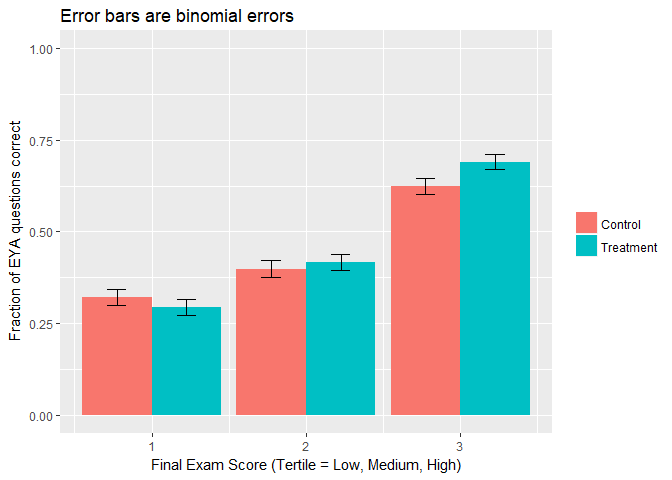
\includegraphics{A01-Logistic_on_final_exam_data_files/figure-latex/unnamed-chunk-15-1.pdf}

\begin{Shaded}
\begin{Highlighting}[]
\NormalTok{s.crtsplit <-}\StringTok{ }\KeywordTok{summarySE}\NormalTok{(dat.trt, }\DataTypeTok{measurevar=}\StringTok{"QCORRECT"}\NormalTok{,}
                              \DataTypeTok{groupvars=}\KeywordTok{c}\NormalTok{(}\StringTok{"CRT.medsplit"}\NormalTok{,}\StringTok{"TREATMENT"}\NormalTok{), }\DataTypeTok{.drop=}\OtherTok{FALSE}\NormalTok{)}
\NormalTok{limits <-}\StringTok{ }\KeywordTok{aes}\NormalTok{(}\DataTypeTok{ymax =}\NormalTok{ QCORRECT }\OperatorTok{+}\StringTok{ }\NormalTok{binomial.error, }\DataTypeTok{ymin =}\NormalTok{ QCORRECT }\OperatorTok{-}\StringTok{ }\NormalTok{binomial.error)}
\CommentTok{#options(repr.plot.width=5, repr.plot.height=3)}

\KeywordTok{ggplot}\NormalTok{(s.crtsplit, }\KeywordTok{aes}\NormalTok{(}\DataTypeTok{x=}\NormalTok{CRT.medsplit, }\DataTypeTok{y=}\NormalTok{QCORRECT, }\DataTypeTok{fill=}\NormalTok{TREATMENT)) }\OperatorTok{+}\StringTok{ }
\StringTok{    }\KeywordTok{geom_bar}\NormalTok{(}\DataTypeTok{stat=}\StringTok{"identity"}\NormalTok{, }\DataTypeTok{position=}\NormalTok{dodge) }\OperatorTok{+}\StringTok{ }
\StringTok{    }\KeywordTok{geom_errorbar}\NormalTok{(limits, }\DataTypeTok{position=}\NormalTok{dodge, }\DataTypeTok{width=}\FloatTok{0.5}\NormalTok{)}
\end{Highlighting}
\end{Shaded}

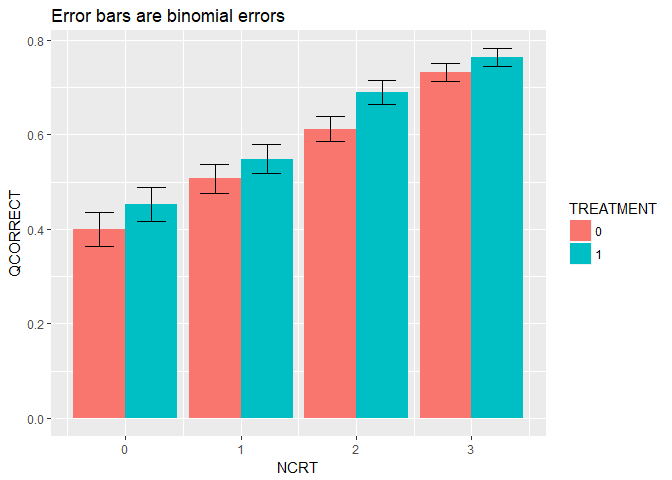
\includegraphics{A01-Logistic_on_final_exam_data_files/figure-latex/unnamed-chunk-16-1.pdf}

\section{And looking at correlations with final exam
grades}\label{and-looking-at-correlations-with-final-exam-grades}

\begin{Shaded}
\begin{Highlighting}[]
\NormalTok{s.fLMH <-}\StringTok{ }\KeywordTok{summarySE}\NormalTok{(dat.trt, }\DataTypeTok{measurevar=}\StringTok{"QCORRECT"}\NormalTok{,}
                              \DataTypeTok{groupvars=}\KeywordTok{c}\NormalTok{(}\StringTok{"final.grade.LMH"}\NormalTok{,}\StringTok{"TREATMENT"}\NormalTok{), }\DataTypeTok{.drop=}\OtherTok{FALSE}\NormalTok{)}
\NormalTok{limits <-}\StringTok{ }\KeywordTok{aes}\NormalTok{(}\DataTypeTok{ymax =}\NormalTok{ QCORRECT }\OperatorTok{+}\StringTok{ }\NormalTok{binomial.error, }\DataTypeTok{ymin =}\NormalTok{ QCORRECT }\OperatorTok{-}\StringTok{ }\NormalTok{binomial.error)}
\CommentTok{#options(repr.plot.width=5, repr.plot.height=3)}

\KeywordTok{ggplot}\NormalTok{(s.fLMH, }\KeywordTok{aes}\NormalTok{(}\DataTypeTok{x=}\NormalTok{final.grade.LMH, }\DataTypeTok{y=}\NormalTok{QCORRECT, }\DataTypeTok{fill=}\NormalTok{TREATMENT)) }\OperatorTok{+}\StringTok{ }
\StringTok{    }\KeywordTok{geom_bar}\NormalTok{(}\DataTypeTok{stat=}\StringTok{"identity"}\NormalTok{, }\DataTypeTok{position=}\NormalTok{dodge) }\OperatorTok{+}\StringTok{ }
\StringTok{    }\KeywordTok{geom_errorbar}\NormalTok{(limits, }\DataTypeTok{position=}\NormalTok{dodge, }\DataTypeTok{width=}\FloatTok{0.5}\NormalTok{)}
\end{Highlighting}
\end{Shaded}

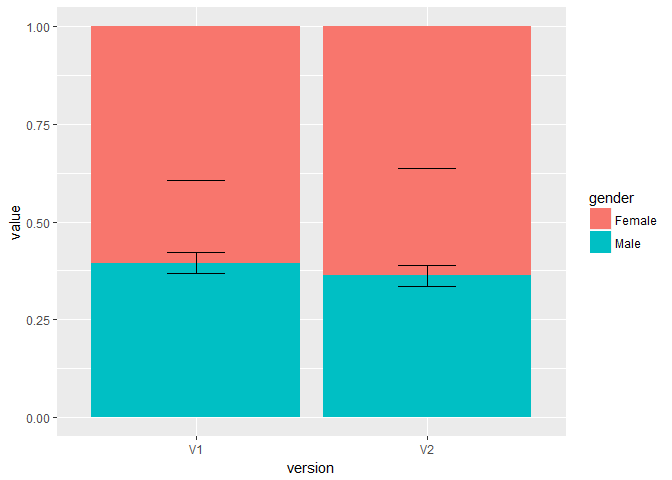
\includegraphics{A01-Logistic_on_final_exam_data_files/figure-latex/unnamed-chunk-17-1.pdf}

\section{Finally, let's look at
gender}\label{finally-lets-look-at-gender}

\subsubsection{Bar graph splitting on gender and looking at the effect
of
treatment}\label{bar-graph-splitting-on-gender-and-looking-at-the-effect-of-treatment}

Splitting on gender shows that there may be a significant difference in
who the intervention helps

\begin{Shaded}
\begin{Highlighting}[]
\NormalTok{sum.gender <-}\StringTok{ }\KeywordTok{summarySE}\NormalTok{(dat.trt, }\DataTypeTok{measurevar=}\StringTok{"QCORRECT"}\NormalTok{,}
                              \DataTypeTok{groupvars=}\KeywordTok{c}\NormalTok{(}\StringTok{"Gender"}\NormalTok{,}\StringTok{"TREATMENT"}\NormalTok{), }\DataTypeTok{.drop=}\OtherTok{FALSE}\NormalTok{)}

\NormalTok{limits <-}\StringTok{ }\KeywordTok{aes}\NormalTok{(}\DataTypeTok{ymax =}\NormalTok{ QCORRECT }\OperatorTok{+}\StringTok{ }\NormalTok{binomial.error, }\DataTypeTok{ymin =}\NormalTok{ QCORRECT }\OperatorTok{-}\StringTok{ }\NormalTok{binomial.error)}

\KeywordTok{ggplot}\NormalTok{(sum.gender, }\KeywordTok{aes}\NormalTok{(}\DataTypeTok{x=}\NormalTok{Gender, }\DataTypeTok{y=}\NormalTok{QCORRECT, }\DataTypeTok{fill=}\NormalTok{TREATMENT)) }\OperatorTok{+}\StringTok{ }
\StringTok{    }\KeywordTok{geom_bar}\NormalTok{(}\DataTypeTok{stat=}\StringTok{"identity"}\NormalTok{, }\DataTypeTok{position=}\NormalTok{dodge) }\OperatorTok{+}\StringTok{ }
\StringTok{    }\KeywordTok{geom_errorbar}\NormalTok{(limits, }\DataTypeTok{position=}\NormalTok{dodge, }\DataTypeTok{width=}\FloatTok{0.5}\NormalTok{)}
\end{Highlighting}
\end{Shaded}

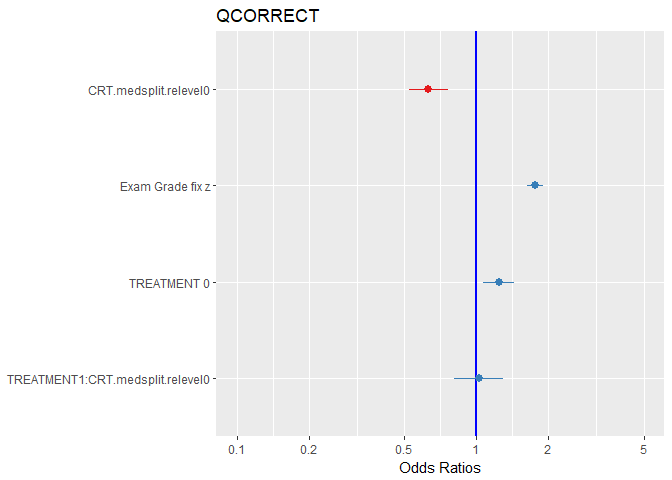
\includegraphics{A01-Logistic_on_final_exam_data_files/figure-latex/unnamed-chunk-18-1.pdf}

\subsubsection{Logistic regression with gender
added}\label{logistic-regression-with-gender-added}

Gender is significant.

\begin{Shaded}
\begin{Highlighting}[]
\NormalTok{m.gender0 <-}\StringTok{ }\KeywordTok{glmer}\NormalTok{(QCORRECT }\OperatorTok{~}\StringTok{ }\NormalTok{QNUM }\OperatorTok{+}\StringTok{ }\NormalTok{TREATMENT }\OperatorTok{+}\StringTok{ }\NormalTok{Gender }\OperatorTok{+}\StringTok{ }\NormalTok{(}\DecValTok{1}\OperatorTok{|}\NormalTok{ID), }
                \DataTypeTok{data =}\NormalTok{ dat.trt, }
                \DataTypeTok{family =}\NormalTok{ binomial, }\DataTypeTok{control=}\KeywordTok{glmerControl}\NormalTok{(}\DataTypeTok{optimizer=}\StringTok{"bobyqa"}\NormalTok{))}
\KeywordTok{summary}\NormalTok{(m.gender0)}
\end{Highlighting}
\end{Shaded}

\begin{verbatim}
## Generalized linear mixed model fit by maximum likelihood (Laplace
##   Approximation) [glmerMod]
##  Family: binomial  ( logit )
## Formula: QCORRECT ~ QNUM + TREATMENT + Gender + (1 | ID)
##    Data: dat.trt
## Control: glmerControl(optimizer = "bobyqa")
## 
##      AIC      BIC   logLik deviance df.resid 
##   3288.5   3329.5  -1637.2   3274.5     2613 
## 
## Scaled residuals: 
##     Min      1Q  Median      3Q     Max 
## -2.2496 -0.9548  0.5067  0.6997  1.4685 
## 
## Random effects:
##  Groups Name        Variance Std.Dev.
##  ID     (Intercept) 0.4913   0.7009  
## Number of obs: 2620, groups:  ID, 658
## 
## Fixed effects:
##              Estimate Std. Error z value Pr(>|z|)    
## (Intercept)  0.567639   0.110691   5.128 2.93e-07 ***
## QNUM6       -0.894988   0.125099  -7.154 8.41e-13 ***
## QNUM9        0.000603   0.128207   0.005  0.99625    
## QNUM10      -0.552625   0.124938  -4.423 9.72e-06 ***
## TREATMENT1   0.250017   0.087757   2.849  0.00439 ** 
## GenderMale   0.793746   0.109970   7.218 5.28e-13 ***
## ---
## Signif. codes:  0 '***' 0.001 '**' 0.01 '*' 0.05 '.' 0.1 ' ' 1
## 
## Correlation of Fixed Effects:
##            (Intr) QNUM6  QNUM9  QNUM10 TREATM
## QNUM6      -0.596                            
## QNUM9      -0.579  0.512                     
## QNUM10     -0.595  0.540  0.513              
## TREATMENT1 -0.381 -0.018  0.002 -0.012       
## GenderMale -0.310 -0.055 -0.001 -0.034  0.024
\end{verbatim}

\subsubsection{Run logistic regressions on the two gender populations
seperately}\label{run-logistic-regressions-on-the-two-gender-populations-seperately}

First without course grades included. Treatment is only significant for
females, not males.

\begin{Shaded}
\begin{Highlighting}[]
\NormalTok{m.female <-}\StringTok{ }\KeywordTok{glmer}\NormalTok{(QCORRECT }\OperatorTok{~}\StringTok{ }\NormalTok{QNUM }\OperatorTok{+}\StringTok{ }\NormalTok{TREATMENT }\OperatorTok{+}\StringTok{ }\NormalTok{(}\DecValTok{1}\OperatorTok{|}\NormalTok{ID), }
                \DataTypeTok{data =} \KeywordTok{subset}\NormalTok{(dat.trt, Gender}\OperatorTok{==}\StringTok{"Female"}\NormalTok{), }
                \DataTypeTok{family =}\NormalTok{ binomial, }\DataTypeTok{control=}\KeywordTok{glmerControl}\NormalTok{(}\DataTypeTok{optimizer=}\StringTok{"bobyqa"}\NormalTok{))}
\KeywordTok{summary}\NormalTok{(m.female)}
\end{Highlighting}
\end{Shaded}

\begin{verbatim}
## Generalized linear mixed model fit by maximum likelihood (Laplace
##   Approximation) [glmerMod]
##  Family: binomial  ( logit )
## Formula: QCORRECT ~ QNUM + TREATMENT + (1 | ID)
##    Data: subset(dat.trt, Gender == "Female")
## Control: glmerControl(optimizer = "bobyqa")
## 
##      AIC      BIC   logLik deviance df.resid 
##   2161.7   2194.1  -1074.9   2149.7     1624 
## 
## Scaled residuals: 
##     Min      1Q  Median      3Q     Max 
## -1.6950 -0.9826  0.5855  0.7996  1.5265 
## 
## Random effects:
##  Groups Name        Variance Std.Dev.
##  ID     (Intercept) 0.4497   0.6706  
## Number of obs: 1630, groups:  ID, 409
## 
## Fixed effects:
##             Estimate Std. Error z value Pr(>|z|)    
## (Intercept)  0.54798    0.12555   4.365 1.27e-05 ***
## QNUM6       -0.97894    0.15394  -6.359 2.03e-10 ***
## QNUM9       -0.01544    0.15396  -0.100  0.92011    
## QNUM10      -0.45561    0.15200  -2.997  0.00272 ** 
## TREATMENT1   0.28553    0.10750   2.656  0.00791 ** 
## ---
## Signif. codes:  0 '***' 0.001 '**' 0.01 '*' 0.05 '.' 0.1 ' ' 1
## 
## Correlation of Fixed Effects:
##            (Intr) QNUM6  QNUM9  QNUM10
## QNUM6      -0.620                     
## QNUM9      -0.614  0.500              
## QNUM10     -0.621  0.521  0.507       
## TREATMENT1 -0.395 -0.045  0.001 -0.029
\end{verbatim}

\begin{Shaded}
\begin{Highlighting}[]
\NormalTok{m<-m.female}
\NormalTok{se <-}\StringTok{ }\KeywordTok{sqrt}\NormalTok{(}\KeywordTok{diag}\NormalTok{(}\KeywordTok{vcov}\NormalTok{(m)))}
\NormalTok{tab <-}\StringTok{ }\KeywordTok{cbind}\NormalTok{(}\DataTypeTok{Est =} \KeywordTok{fixef}\NormalTok{(m), }\DataTypeTok{LL =} \KeywordTok{fixef}\NormalTok{(m) }\OperatorTok{-}\StringTok{ }\FloatTok{1.96} \OperatorTok{*}\StringTok{ }\NormalTok{se, }\DataTypeTok{UL =} \KeywordTok{fixef}\NormalTok{(m) }\OperatorTok{+}\StringTok{ }\FloatTok{1.96} \OperatorTok{*}\NormalTok{se)}
\KeywordTok{exp}\NormalTok{(tab)}
\end{Highlighting}
\end{Shaded}

\begin{verbatim}
##                   Est        LL        UL
## (Intercept) 1.7297536 1.3524364 2.2123388
## QNUM6       0.3757092 0.2778549 0.5080255
## QNUM9       0.9846771 0.7281771 1.3315293
## QNUM10      0.6340631 0.4707062 0.8541124
## TREATMENT1  1.3304630 1.0776980 1.6425120
\end{verbatim}

\begin{Shaded}
\begin{Highlighting}[]
\NormalTok{m.male <-}\StringTok{ }\KeywordTok{glmer}\NormalTok{(QCORRECT }\OperatorTok{~}\StringTok{ }\NormalTok{QNUM }\OperatorTok{+}\StringTok{ }\NormalTok{TREATMENT }\OperatorTok{+}\StringTok{ }\NormalTok{(}\DecValTok{1}\OperatorTok{|}\NormalTok{ID), }
                \DataTypeTok{data =} \KeywordTok{subset}\NormalTok{(dat.trt, Gender}\OperatorTok{==}\StringTok{"Male"}\NormalTok{), }
                \DataTypeTok{family =}\NormalTok{ binomial, }\DataTypeTok{control=}\KeywordTok{glmerControl}\NormalTok{(}\DataTypeTok{optimizer=}\StringTok{"bobyqa"}\NormalTok{))}
\KeywordTok{summary}\NormalTok{(m.male)}
\end{Highlighting}
\end{Shaded}

\begin{verbatim}
## Generalized linear mixed model fit by maximum likelihood (Laplace
##   Approximation) [glmerMod]
##  Family: binomial  ( logit )
## Formula: QCORRECT ~ QNUM + TREATMENT + (1 | ID)
##    Data: subset(dat.trt, Gender == "Male")
## Control: glmerControl(optimizer = "bobyqa")
## 
##      AIC      BIC   logLik deviance df.resid 
##   1131.6   1161.0   -559.8   1119.6      984 
## 
## Scaled residuals: 
##     Min      1Q  Median      3Q     Max 
## -2.2693 -0.9380  0.4490  0.5734  1.0613 
## 
## Random effects:
##  Groups Name        Variance Std.Dev.
##  ID     (Intercept) 0.6002   0.7747  
## Number of obs: 990, groups:  ID, 249
## 
## Fixed effects:
##             Estimate Std. Error z value Pr(>|z|)    
## (Intercept)  1.42031    0.19600   7.246 4.28e-13 ***
## QNUM6       -0.75169    0.21979  -3.420 0.000626 ***
## QNUM9        0.03745    0.23347   0.160 0.872557    
## QNUM10      -0.74281    0.21958  -3.383 0.000717 ***
## TREATMENT1   0.17833    0.15375   1.160 0.246091    
## ---
## Signif. codes:  0 '***' 0.001 '**' 0.01 '*' 0.05 '.' 0.1 ' ' 1
## 
## Correlation of Fixed Effects:
##            (Intr) QNUM6  QNUM9  QNUM10
## QNUM6      -0.674                     
## QNUM9      -0.591  0.527              
## QNUM10     -0.672  0.575  0.528       
## TREATMENT1 -0.392  0.032  0.005  0.028
\end{verbatim}

\begin{Shaded}
\begin{Highlighting}[]
\NormalTok{m<-m.male}
\NormalTok{se <-}\StringTok{ }\KeywordTok{sqrt}\NormalTok{(}\KeywordTok{diag}\NormalTok{(}\KeywordTok{vcov}\NormalTok{(m)))}
\NormalTok{tab <-}\StringTok{ }\KeywordTok{cbind}\NormalTok{(}\DataTypeTok{Est =} \KeywordTok{fixef}\NormalTok{(m), }\DataTypeTok{LL =} \KeywordTok{fixef}\NormalTok{(m) }\OperatorTok{-}\StringTok{ }\FloatTok{1.96} \OperatorTok{*}\StringTok{ }\NormalTok{se, }\DataTypeTok{UL =} \KeywordTok{fixef}\NormalTok{(m) }\OperatorTok{+}\StringTok{ }\FloatTok{1.96} \OperatorTok{*}\NormalTok{se)}
\KeywordTok{exp}\NormalTok{(tab)}
\end{Highlighting}
\end{Shaded}

\begin{verbatim}
##                   Est        LL        UL
## (Intercept) 4.1384133 2.8183316 6.0768095
## QNUM6       0.4715667 0.3065180 0.7254882
## QNUM9       1.0381613 0.6569490 1.6405823
## QNUM10      0.4757749 0.3093769 0.7316696
## TREATMENT1  1.1952190 0.8842524 1.6155439
\end{verbatim}

When controlling for course grade, nothing changes

\begin{Shaded}
\begin{Highlighting}[]
\NormalTok{m.female.grade <-}\StringTok{ }\KeywordTok{glmer}\NormalTok{(QCORRECT }\OperatorTok{~}\StringTok{ }\NormalTok{QNUM }\OperatorTok{+}\StringTok{ }\NormalTok{TREATMENT }\OperatorTok{+}\StringTok{ }\NormalTok{course.grade.frac }\OperatorTok{+}\StringTok{ }\NormalTok{(}\DecValTok{1}\OperatorTok{|}\NormalTok{ID), }
                \DataTypeTok{data =} \KeywordTok{subset}\NormalTok{(dat.trt,Gender}\OperatorTok{==}\StringTok{"Female"}\NormalTok{), }
                \DataTypeTok{family =}\NormalTok{ binomial, }\DataTypeTok{control=}\KeywordTok{glmerControl}\NormalTok{(}\DataTypeTok{optimizer=}\StringTok{"bobyqa"}\NormalTok{))}
\KeywordTok{summary}\NormalTok{(m.female.grade)}
\end{Highlighting}
\end{Shaded}

\begin{verbatim}
## Generalized linear mixed model fit by maximum likelihood (Laplace
##   Approximation) [glmerMod]
##  Family: binomial  ( logit )
## Formula: QCORRECT ~ QNUM + TREATMENT + course.grade.frac + (1 | ID)
##    Data: subset(dat.trt, Gender == "Female")
## Control: glmerControl(optimizer = "bobyqa")
## 
##      AIC      BIC   logLik deviance df.resid 
##   2030.9   2068.7  -1008.5   2016.9     1623 
## 
## Scaled residuals: 
##     Min      1Q  Median      3Q     Max 
## -2.1171 -0.9385  0.4891  0.7533  2.4850 
## 
## Random effects:
##  Groups Name        Variance Std.Dev.
##  ID     (Intercept) 0.06234  0.2497  
## Number of obs: 1630, groups:  ID, 409
## 
## Fixed effects:
##                   Estimate Std. Error z value Pr(>|z|)    
## (Intercept)        -3.2475     0.3539  -9.177  < 2e-16 ***
## QNUM6              -0.9817     0.1543  -6.363 1.98e-10 ***
## QNUM9              -0.0142     0.1553  -0.091  0.92714    
## QNUM10             -0.4558     0.1528  -2.983  0.00285 ** 
## TREATMENT1          0.2801     0.1079   2.596  0.00944 ** 
## course.grade.frac   5.2249     0.4699  11.119  < 2e-16 ***
## ---
## Signif. codes:  0 '***' 0.001 '**' 0.01 '*' 0.05 '.' 0.1 ' ' 1
## 
## Correlation of Fixed Effects:
##             (Intr) QNUM6  QNUM9  QNUM10 TREATM
## QNUM6       -0.114                            
## QNUM9       -0.219  0.503                     
## QNUM10      -0.174  0.523  0.508              
## TREATMENT1  -0.176 -0.035  0.001 -0.020       
## crs.grd.frc -0.938 -0.114 -0.001 -0.051  0.035
\end{verbatim}

\begin{Shaded}
\begin{Highlighting}[]
\NormalTok{m.male.grade <-}\StringTok{ }\KeywordTok{glmer}\NormalTok{(QCORRECT }\OperatorTok{~}\StringTok{ }\NormalTok{QNUM }\OperatorTok{+}\StringTok{ }\NormalTok{TREATMENT }\OperatorTok{+}\StringTok{ }\NormalTok{course.grade.frac }\OperatorTok{+}\StringTok{ }\NormalTok{(}\DecValTok{1}\OperatorTok{|}\NormalTok{ID), }
                \DataTypeTok{data =} \KeywordTok{subset}\NormalTok{(dat.trt,Gender}\OperatorTok{==}\StringTok{"Male"}\NormalTok{), }
                \DataTypeTok{family =}\NormalTok{ binomial, }\DataTypeTok{control=}\KeywordTok{glmerControl}\NormalTok{(}\DataTypeTok{optimizer=}\StringTok{"bobyqa"}\NormalTok{))}
\KeywordTok{summary}\NormalTok{(m.male.grade)}
\end{Highlighting}
\end{Shaded}

\begin{verbatim}
## Generalized linear mixed model fit by maximum likelihood (Laplace
##   Approximation) [glmerMod]
##  Family: binomial  ( logit )
## Formula: QCORRECT ~ QNUM + TREATMENT + course.grade.frac + (1 | ID)
##    Data: subset(dat.trt, Gender == "Male")
## Control: glmerControl(optimizer = "bobyqa")
## 
##      AIC      BIC   logLik deviance df.resid 
##   1032.8   1067.1   -509.4   1018.8      983 
## 
## Scaled residuals: 
##     Min      1Q  Median      3Q     Max 
## -3.5741 -0.5821  0.4021  0.5685  1.9337 
## 
## Random effects:
##  Groups Name        Variance Std.Dev.
##  ID     (Intercept) 0.03624  0.1904  
## Number of obs: 990, groups:  ID, 249
## 
## Fixed effects:
##                   Estimate Std. Error z value Pr(>|z|)    
## (Intercept)        -3.3260     0.5009  -6.640 3.13e-11 ***
## QNUM6              -0.7723     0.2232  -3.461 0.000539 ***
## QNUM9               0.0467     0.2383   0.196 0.844641    
## QNUM10             -0.7580     0.2230  -3.399 0.000676 ***
## TREATMENT1          0.1741     0.1555   1.119 0.263030    
## course.grade.frac   6.1641     0.6521   9.453  < 2e-16 ***
## ---
## Signif. codes:  0 '***' 0.001 '**' 0.01 '*' 0.05 '.' 0.1 ' ' 1
## 
## Correlation of Fixed Effects:
##             (Intr) QNUM6  QNUM9  QNUM10 TREATM
## QNUM6       -0.166                            
## QNUM9       -0.247  0.528                     
## QNUM10      -0.170  0.581  0.529              
## TREATMENT1  -0.180  0.044  0.006  0.040       
## crs.grd.frc -0.926 -0.104  0.011 -0.099  0.020
\end{verbatim}

\subsubsection{Looking at interaction
term}\label{looking-at-interaction-term}

\begin{Shaded}
\begin{Highlighting}[]
\NormalTok{m.gender <-}\StringTok{ }\KeywordTok{glmer}\NormalTok{(QCORRECT }\OperatorTok{~}\StringTok{ }\NormalTok{QNUM }\OperatorTok{+}\StringTok{ }\NormalTok{TREATMENT}\OperatorTok{*}\NormalTok{Gender }\OperatorTok{+}\StringTok{ }\NormalTok{(}\DecValTok{1}\OperatorTok{|}\NormalTok{ID), }
                \DataTypeTok{data =}\NormalTok{ dat.trt, }
                \DataTypeTok{family =}\NormalTok{ binomial, }\DataTypeTok{control=}\KeywordTok{glmerControl}\NormalTok{(}\DataTypeTok{optimizer=}\StringTok{"bobyqa"}\NormalTok{))}
\KeywordTok{summary}\NormalTok{(m.gender)}
\end{Highlighting}
\end{Shaded}

\begin{verbatim}
## Generalized linear mixed model fit by maximum likelihood (Laplace
##   Approximation) [glmerMod]
##  Family: binomial  ( logit )
## Formula: QCORRECT ~ QNUM + TREATMENT * Gender + (1 | ID)
##    Data: dat.trt
## Control: glmerControl(optimizer = "bobyqa")
## 
##      AIC      BIC   logLik deviance df.resid 
##   3290.1   3337.1  -1637.0   3274.1     2612 
## 
## Scaled residuals: 
##     Min      1Q  Median      3Q     Max 
## -2.2060 -0.9461  0.4972  0.6930  1.4834 
## 
## Random effects:
##  Groups Name        Variance Std.Dev.
##  ID     (Intercept) 0.492    0.7014  
## Number of obs: 2620, groups:  ID, 658
## 
## Fixed effects:
##                         Estimate Std. Error z value Pr(>|z|)    
## (Intercept)            0.5505355  0.1143230   4.816 1.47e-06 ***
## QNUM6                 -0.8972681  0.1251816  -7.168 7.62e-13 ***
## QNUM9                  0.0004719  0.1282263   0.004  0.99706    
## QNUM10                -0.5546810  0.1250070  -4.437 9.11e-06 ***
## TREATMENT1             0.2870489  0.1076585   2.666  0.00767 ** 
## GenderMale             0.8476396  0.1425759   5.945 2.76e-09 ***
## TREATMENT1:GenderMale -0.1110428  0.1858459  -0.597  0.55017    
## ---
## Signif. codes:  0 '***' 0.001 '**' 0.01 '*' 0.05 '.' 0.1 ' ' 1
## 
## Correlation of Fixed Effects:
##             (Intr) QNUM6  QNUM9  QNUM10 TREATMENT1 GndrMl
## QNUM6       -0.568                                       
## QNUM9       -0.561  0.512                                
## QNUM10      -0.568  0.540  0.513                         
## TREATMENT1  -0.445 -0.034  0.001 -0.026                  
## GenderMale  -0.389 -0.064 -0.002 -0.045  0.380           
## TREATMENT1:  0.250  0.033  0.002  0.029 -0.579     -0.636
\end{verbatim}

\begin{Shaded}
\begin{Highlighting}[]
\NormalTok{m<-m.gender}
\NormalTok{se <-}\StringTok{ }\KeywordTok{sqrt}\NormalTok{(}\KeywordTok{diag}\NormalTok{(}\KeywordTok{vcov}\NormalTok{(m)))}
\NormalTok{tab <-}\StringTok{ }\KeywordTok{cbind}\NormalTok{(}\DataTypeTok{Est =} \KeywordTok{fixef}\NormalTok{(m), }\DataTypeTok{LL =} \KeywordTok{fixef}\NormalTok{(m) }\OperatorTok{-}\StringTok{ }\FloatTok{1.96} \OperatorTok{*}\StringTok{ }\NormalTok{se, }\DataTypeTok{UL =} \KeywordTok{fixef}\NormalTok{(m) }\OperatorTok{+}\StringTok{ }\FloatTok{1.96} \OperatorTok{*}\NormalTok{se)}
\KeywordTok{exp}\NormalTok{(tab)}
\end{Highlighting}
\end{Shaded}

\begin{verbatim}
##                             Est        LL        UL
## (Intercept)           1.7341814 1.3860560 2.1697428
## QNUM6                 0.4076819 0.3189809 0.5210485
## QNUM9                 1.0004720 0.7781378 1.2863328
## QNUM10                0.5742554 0.4494662 0.7336911
## TREATMENT1            1.3324893 1.0790039 1.6455250
## GenderMale            2.3341308 1.7650709 3.0866560
## TREATMENT1:GenderMale 0.8949005 0.6216980 1.2881605
\end{verbatim}

\subsubsection{Control for overall exam score (yes, re-calcuated for
each question to not include the specific question in the
score)}\label{control-for-overall-exam-score-yes-re-calcuated-for-each-question-to-not-include-the-specific-question-in-the-score}

Treatment does not change significantly, but when controlling for final
exam score the gender effect goes down significantly

\begin{Shaded}
\begin{Highlighting}[]
\NormalTok{m.fgradeA <-}\StringTok{ }\KeywordTok{glmer}\NormalTok{(QCORRECT }\OperatorTok{~}\StringTok{ }\NormalTok{QNUM }\OperatorTok{+}\StringTok{ }\NormalTok{TREATMENT }\OperatorTok{+}\StringTok{ }\NormalTok{final.gradeA.fix }\OperatorTok{+}\StringTok{ }\NormalTok{Gender }\OperatorTok{+}\StringTok{ }\NormalTok{(}\DecValTok{1}\OperatorTok{|}\NormalTok{ID), }
                \DataTypeTok{data =}\NormalTok{ dat.trt, }
                \DataTypeTok{family =}\NormalTok{ binomial, }\DataTypeTok{control=}\KeywordTok{glmerControl}\NormalTok{(}\DataTypeTok{optimizer=}\StringTok{"bobyqa"}\NormalTok{))}
\KeywordTok{summary}\NormalTok{(m.fgradeA)}
\end{Highlighting}
\end{Shaded}

\begin{verbatim}
## Generalized linear mixed model fit by maximum likelihood (Laplace
##   Approximation) [glmerMod]
##  Family: binomial  ( logit )
## Formula: QCORRECT ~ QNUM + TREATMENT + final.gradeA.fix + Gender + (1 |  
##     ID)
##    Data: dat.trt
## Control: glmerControl(optimizer = "bobyqa")
## 
##      AIC      BIC   logLik deviance df.resid 
##   3143.2   3190.1  -1563.6   3127.2     2612 
## 
## Scaled residuals: 
##     Min      1Q  Median      3Q     Max 
## -3.3088 -0.9548  0.4817  0.7213  2.3850 
## 
## Random effects:
##  Groups Name        Variance Std.Dev.
##  ID     (Intercept) 0        0       
## Number of obs: 2620, groups:  ID, 658
## 
## Fixed effects:
##                  Estimate Std. Error z value Pr(>|z|)    
## (Intercept)      -1.42511    0.17934  -7.947 1.92e-15 ***
## QNUM6            -0.89729    0.12255  -7.322 2.45e-13 ***
## QNUM9             0.00104    0.12683   0.008  0.99346    
## QNUM10           -0.55284    0.12312  -4.490 7.12e-06 ***
## TREATMENT1        0.24743    0.08636   2.865  0.00417 ** 
## final.gradeA.fix  3.19745    0.24744  12.922  < 2e-16 ***
## GenderMale        0.49859    0.09281   5.372 7.79e-08 ***
## ---
## Signif. codes:  0 '***' 0.001 '**' 0.01 '*' 0.05 '.' 0.1 ' ' 1
## 
## Correlation of Fixed Effects:
##             (Intr) QNUM6  QNUM9  QNUM10 TREATM fnl.A.
## QNUM6       -0.281                                   
## QNUM9       -0.355  0.518                            
## QNUM10      -0.315  0.540  0.515                     
## TREATMENT1  -0.258 -0.008  0.003 -0.003              
## fnl.grdA.fx -0.818 -0.094  0.001 -0.054  0.026       
## GenderMale  -0.032 -0.030 -0.002 -0.019  0.015 -0.156
\end{verbatim}

\begin{Shaded}
\begin{Highlighting}[]
\NormalTok{m.fgrade <-}\StringTok{ }\KeywordTok{glmer}\NormalTok{(QCORRECT }\OperatorTok{~}\StringTok{ }\NormalTok{QNUM }\OperatorTok{+}\StringTok{ }\NormalTok{TREATMENT }\OperatorTok{+}\StringTok{ }\NormalTok{final.grade.fix }\OperatorTok{+}\StringTok{ }\NormalTok{Gender }\OperatorTok{+}\StringTok{ }\NormalTok{(}\DecValTok{1}\OperatorTok{|}\NormalTok{ID), }
                \DataTypeTok{data =}\NormalTok{ dat.trt, }
                \DataTypeTok{family =}\NormalTok{ binomial, }\DataTypeTok{control=}\KeywordTok{glmerControl}\NormalTok{(}\DataTypeTok{optimizer=}\StringTok{"bobyqa"}\NormalTok{))}
\KeywordTok{summary}\NormalTok{(m.fgrade)}
\end{Highlighting}
\end{Shaded}

\begin{verbatim}
## Generalized linear mixed model fit by maximum likelihood (Laplace
##   Approximation) [glmerMod]
##  Family: binomial  ( logit )
## Formula: QCORRECT ~ QNUM + TREATMENT + final.grade.fix + Gender + (1 |  
##     ID)
##    Data: dat.trt
## Control: glmerControl(optimizer = "bobyqa")
## 
##      AIC      BIC   logLik deviance df.resid 
##   3104.2   3151.1  -1544.1   3088.2     2612 
## 
## Scaled residuals: 
##     Min      1Q  Median      3Q     Max 
## -3.4428 -0.9306  0.4630  0.7092  2.5240 
## 
## Random effects:
##  Groups Name        Variance  Std.Dev. 
##  ID     (Intercept) 1.148e-14 1.072e-07
## Number of obs: 2620, groups:  ID, 658
## 
## Fixed effects:
##                  Estimate Std. Error z value Pr(>|z|)    
## (Intercept)     -1.812548   0.191717  -9.454  < 2e-16 ***
## QNUM6           -0.896874   0.123500  -7.262 3.81e-13 ***
## QNUM9            0.001575   0.127780   0.012    0.990    
## QNUM10          -0.552219   0.124039  -4.452 8.51e-06 ***
## TREATMENT1       0.244337   0.087036   2.807    0.005 ** 
## final.grade.fix  3.729663   0.263766  14.140  < 2e-16 ***
## GenderMale       0.505817   0.093251   5.424 5.82e-08 ***
## ---
## Signif. codes:  0 '***' 0.001 '**' 0.01 '*' 0.05 '.' 0.1 ' ' 1
## 
## Correlation of Fixed Effects:
##             (Intr) QNUM6  QNUM9  QNUM10 TREATM fnl.g.
## QNUM6       -0.261                                   
## QNUM9       -0.335  0.517                            
## QNUM10      -0.295  0.539  0.515                     
## TREATMENT1  -0.245 -0.005  0.003  0.000              
## finl.grd.fx -0.840 -0.092  0.001 -0.053  0.024       
## GenderMale  -0.044 -0.031 -0.002 -0.020  0.015 -0.126
\end{verbatim}

\begin{Shaded}
\begin{Highlighting}[]
\NormalTok{m.fgrade.int <-}\StringTok{ }\KeywordTok{glmer}\NormalTok{(QCORRECT }\OperatorTok{~}\StringTok{ }\NormalTok{QNUM }\OperatorTok{+}\StringTok{ }\NormalTok{TREATMENT}\OperatorTok{*}\NormalTok{Gender }\OperatorTok{+}\StringTok{ }\NormalTok{final.grade.fix }\OperatorTok{+}\StringTok{ }\NormalTok{(}\DecValTok{1}\OperatorTok{|}\NormalTok{ID), }
                \DataTypeTok{data =}\NormalTok{ dat.trt, }
                \DataTypeTok{family =}\NormalTok{ binomial, }\DataTypeTok{control=}\KeywordTok{glmerControl}\NormalTok{(}\DataTypeTok{optimizer=}\StringTok{"bobyqa"}\NormalTok{))}
\KeywordTok{summary}\NormalTok{(m.fgrade.int)}
\end{Highlighting}
\end{Shaded}

\begin{verbatim}
## Generalized linear mixed model fit by maximum likelihood (Laplace
##   Approximation) [glmerMod]
##  Family: binomial  ( logit )
## Formula: QCORRECT ~ QNUM + TREATMENT * Gender + final.grade.fix + (1 |  
##     ID)
##    Data: dat.trt
## Control: glmerControl(optimizer = "bobyqa")
## 
##      AIC      BIC   logLik deviance df.resid 
##   3105.9   3158.7  -1543.9   3087.9     2611 
## 
## Scaled residuals: 
##     Min      1Q  Median      3Q     Max 
## -3.3826 -0.9246  0.4642  0.7075  2.5032 
## 
## Random effects:
##  Groups Name        Variance  Std.Dev. 
##  ID     (Intercept) 4.702e-14 2.169e-07
## Number of obs: 2620, groups:  ID, 658
## 
## Fixed effects:
##                       Estimate Std. Error z value Pr(>|z|)    
## (Intercept)           -1.82838    0.19383  -9.433  < 2e-16 ***
## QNUM6                 -0.89881    0.12357  -7.274 3.49e-13 ***
## QNUM9                  0.00138    0.12780   0.011  0.99138    
## QNUM10                -0.55398    0.12410  -4.464 8.04e-06 ***
## TREATMENT1             0.27866    0.10650   2.617  0.00888 ** 
## GenderMale             0.55597    0.12951   4.293 1.76e-05 ***
## final.grade.fix        3.72950    0.26371  14.142  < 2e-16 ***
## TREATMENT1:GenderMale -0.10353    0.18490  -0.560  0.57552    
## ---
## Signif. codes:  0 '***' 0.001 '**' 0.01 '*' 0.05 '.' 0.1 ' ' 1
## 
## Correlation of Fixed Effects:
##             (Intr) QNUM6  QNUM9  QNUM10 TREATMENT1 GndrMl fnl.g.
## QNUM6       -0.254                                              
## QNUM9       -0.331  0.517                                       
## QNUM10      -0.288  0.539  0.515                                
## TREATMENT1  -0.283 -0.021  0.001 -0.015                         
## GenderMale  -0.133 -0.043 -0.003 -0.033  0.405                  
## finl.grd.fx -0.831 -0.092  0.001 -0.053  0.021     -0.089       
## TREATMENT1:  0.148  0.030  0.003  0.026 -0.576     -0.694 -0.002
\end{verbatim}

\begin{Shaded}
\begin{Highlighting}[]
\NormalTok{m<-m.fgrade.int}
\NormalTok{se <-}\StringTok{ }\KeywordTok{sqrt}\NormalTok{(}\KeywordTok{diag}\NormalTok{(}\KeywordTok{vcov}\NormalTok{(m)))}
\NormalTok{tab <-}\StringTok{ }\KeywordTok{cbind}\NormalTok{(}\DataTypeTok{Est =} \KeywordTok{fixef}\NormalTok{(m), }\DataTypeTok{LL =} \KeywordTok{fixef}\NormalTok{(m) }\OperatorTok{-}\StringTok{ }\FloatTok{1.96} \OperatorTok{*}\StringTok{ }\NormalTok{se, }\DataTypeTok{UL =} \KeywordTok{fixef}\NormalTok{(m) }\OperatorTok{+}\StringTok{ }\FloatTok{1.96} \OperatorTok{*}\NormalTok{se)}
\KeywordTok{exp}\NormalTok{(tab)}
\end{Highlighting}
\end{Shaded}

\begin{verbatim}
##                              Est         LL         UL
## (Intercept)            0.1606736  0.1098881  0.2349299
## QNUM6                  0.4070535  0.3194996  0.5186002
## QNUM9                  1.0013810  0.7794947  1.2864283
## QNUM10                 0.5746600  0.4505866  0.7328982
## TREATMENT1             1.3213578  1.0724332  1.6280608
## GenderMale             1.7436241  1.3527281  2.2474767
## final.grade.fix       41.6582357 24.8442523 69.8515124
## TREATMENT1:GenderMale  0.9016484  0.6275512  1.2954637
\end{verbatim}


\end{document}
